\documentclass[11pt]{article}

%We want to be wider
\usepackage{a4wide}
\usepackage{wrapfig}
\usepackage{tikz}

% Input encoding
\usepackage[utf8]{inputenc}
\usepackage{eurosym}
\usepackage{placeins}

\usepackage{caption}
\usepackage{subcaption}

%Syntax Highlighting
\usepackage{listings}

\usepackage{color}
\definecolor{gray}{rgb}{0.4,0.4,0.4}
\definecolor{darkblue}{rgb}{0.0,0.0,0.6}
\definecolor{cyan}{rgb}{0.0,0.6,0.6}

\lstset{
  basicstyle=\ttfamily,
  columns=fullflexible,
  showstringspaces=false,
  commentstyle=\color{gray}\upshape
}

\lstdefinelanguage{XML}
{
  morestring=[b]",
  morestring=[s]{>}{<},
  morecomment=[s]{<?}{?>},
  stringstyle=\color{black},
  identifierstyle=\color{darkblue},
  keywordstyle=\color{cyan},
  morekeywords={xmlns,version,type}% list your attributes here
}

\usepackage{color}

% Math packages
\usepackage{amsfonts}
\usepackage{amssymb}
\usepackage{amsmath}

%Add some color
\usepackage{xcolor}

% WE want colored links instead of ugly boxes
\usepackage[colorlinks=true]{hyperref}
\usepackage{url}

% Ednotes
\usepackage[show]{ed}


% BibTex
\usepackage{cite}

\title{KAT: an Annotation Tool for STEM Documents}
\author{Sourabh Lal, Michael Kohlhase, Tom Wiesing}

\date{\today}

\begin{document}

%Title Page
\maketitle

%The abstract
\begin{abstract}
  Contemporary natural language processing (NLP) systems are based on corpora of annotated
  documents for training and evaluation. To extend NLP to documents from Science,
  Technology, Engineering, and Mathematics (STEM) we need annotation systems that can deal
  with structured elements like mathematical formulae, tables, and possibly even
  diagrams. Current linguistic annotation systems treat documents as word sequences and
  disregard the structure of complex document elements, and are therefore unsuited for
  STEM annotation as this very structure carries important syntactic and semantic
  information.

  We present the KAT system, a browser-based annotation tool for linguistic/semantic
  annotations in structured (XHTML5, i.e. HTML + MathML + SVG in XML serialization)
  documents. As KAT is parametric in the annotation ontology and represents annotations as
  RDF, it can easily be integrated into RDF-based corpus management systems; we present an
  integration into the CorTeX system.
\end{abstract}

\tableofcontents

\section{Introduction}
What is KAT for?
What annot are there?
Sourabh

\section{State Of The Art}
	Currently there are several annotations tools available to use for online text annotations including Hypothes.is, brat, Yawas and Annotatie \cite{stateOfTheArt}. Most state of the art anotation tools create one of the following types of annotations: \ednote{decide whether to put his in intro or here}
	  \begin{enumerate}
	    \item \textit{Dynamic Annotations} - These create annotations that are anchored to the text of the document.
	    \item \textit{Static Annotations} - These create annotations that are anchored to a particular position in the page of the document.
	  \end{enumerate}

	\subsection{Hypothes.is}
    	Hypothes.is \cite{hypothesis} is a tool developed with the aim of ``adding a new layer to the web''. This tool is an online, dynamic annotation tool that can highlight and annotate pdfs and web pages. It provides additional features such as the ability to make an annotation public or private, and being able to post replies to annotations. A user needs to create an account before they can create an annotation, enabling Hypothes.is to show the user his/her private annotations each time they access the webpage. The tool can be either downloaded or run as a Javascript plugin.    

    \subsection{brat}
	    The brat rapid annotation tool \cite{brat} is a web based dynamic text annotation tool. It is designed to create annotations that have a fixed form that can be automatically processed and interpreted. brat can handle two basic types of annotations:
	    \begin{enumerate}
	      \item Text Span Annotations: Creates a simple annotation on a stretch of highlighted text.
	      \item Relation Annotations: Creates a connection between two text-span annotations.
	    \end{enumerate}

	    brat provides several functionalities that make it easy to use. The main ones are:
	    \begin{enumerate}
	      \item Advanced annotation searching tool.
	      \item An annotation export interface that can convert the internal storage format to PDF or HTML.
	      \item Unique address to access each annotation.
	    \end{enumerate}

  	\subsection{Weaknesses Identified in SotA}
    	\paragraph{Inability to handle structured documents}
    		When creating a new annotation, we need to mark the text that the annotation refers to. The state of the art annotation tools are equipped to handle only plain-text documents. While this makes storing annotations very simple as we just store the positions of the start and end characters in a string, it also makes it unsuitable for STEM annotation as the structure carries important syntactic and semantic information
    	\paragraph{Visually disruptive annotations}
    		One key weakness with state of the art annotation tools is the fact that certain annotations break the flow of the underlying text. This is particularly true of relation annotations in brat. If there are several relation annotations connecting two annotations that are separated by a multiple lines, the layout of the document is no longer user friendly.
    	\paragraph{Insufficient help for new users}
    		In order to improve user experience and system usability there needs to be more help provided to help new users understand how to use the new system. While brat provided a tutorial, none of the other 3 systems had any sort of help or guide. Yet even in brat, finding the tutorial was not intuitive.
\section{The KAT System Architecture \& Implementation}

\begin{wrapfigure}r{7.6cm}\vspace*{-2em}
  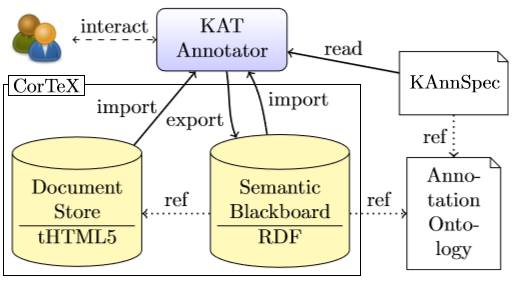
\includegraphics[width=7.6cm]{img/arch}
  \caption{The KAT System Architecture}\label{fig:kat-arch}\vspace*{-1em}
\end{wrapfigure}


As KAT is based on XHTML5, we can employ the XML tool chain and rely on standard libraries for the implementation. In particular, we can use uniform resource identifiers (URI) to identify text fragments and represent annotations in RDF -- subject/predicate/object triples where the components are URI references to web resources. The subjects are usually text fragments, the objects are as well (for relational annotations) or alternatively are concepts from an annotation ontology (for classificational annotations). The predicates are always properties and relations defined in the annotation ontology.

The KAT system itself is realized as a JavaScript library which instruments an XHTML5 document in a browser. To simplify the URI-based referencing of text ranges (node-sets in the HTML document object model) KAT assumes that the document has been word- and sentence-tokenized; the tokens are wrapped in HTML \textsf{span} elements that carry unique \textsf{id} attributes corresponding to the TEI guidelines. The annotation workflow itself is form-based as shown in Figure~\ref{fig:kat-annotate}: the annotator selects a text range, and is then given a modal form to fill classifications and relations as required by the annotation ontology. The annotations are stored as RDF triples in the browser's local storage and can be visualized by special pop-ups and arrows (see Figure~\ref{fig:kat-annotate}).

\begin{figure}[ht]\centering
  %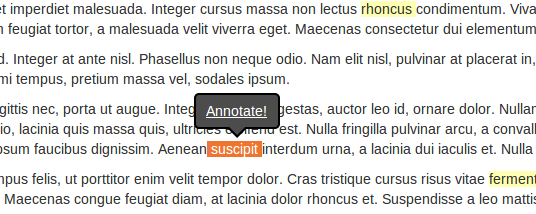
\includegraphics[height=3.2cm]{../papers/PIC/annotate}\quad
  %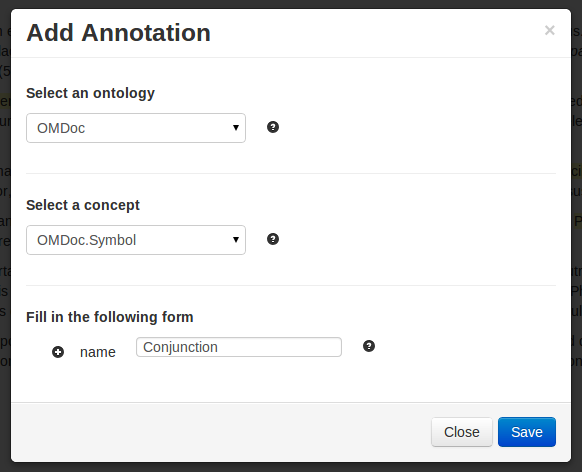
\includegraphics[height=3.1cm]{../papers/PIC/add-symbol}
  \caption{Annotating in KAT: Selection and Form-Filling}\label{fig:kat-annotate}
\end{figure}

KAT is not tied to a particular annotation ontology (or ontology format). At startup, the system is reads a set of \textit{KAT bindings} -- custom XML files that describe the annotation interface, the constraints between the components of an annotation frame, and the RDF to be produced. The frame of OMDoc symbols used in Figure~\ref{fig:kat-annotate}, is given by the fragment of a KAT binding in Listing~\ref{lst:frame}. It specifies
\begin{inparaenum}[\em i\rm)]
\item the fields of the annotation form, their values and validation constraints,
\item their display, and
\item the RDF subgraph for the frame via a templating mechanism.
\end{inparaenum}
Note that this frame classifies the annotated word as an OMDoc symbol (via the \lstinline [basicstyle=\sf\normalsize]|rdf:type| predicate) and relates it to its name via the \lstinline[basicstyle=\sf\normalsize]|o:symbolname| relation from the OMDoc ontology.

\begin{lstlisting}[language=XML,label=lst:frame,
caption=A KAT Frame Specification for OMDoc Symbols]
<frame name="Symbol">
    <help>An OpenMath/OMDoc Symbol</help>
    <fields>
        <field name="name" type="text">
            <help>The name of the symbol defines it in a theory</help>
            <value>Name</value>
            <default>Symbol</default>
            <validation>[A-Z][a-z]*</validation>
        </field>
    </fields>
    <display> ... </display>
    <rdf:RDF xmlns:rdf="http://www.w3.org/1999/02/22-rdf-syntax-ns#">
        <rdf:Description xmlns:o="http://omdoc.org/ontology#">
            <rdf:type rdf:resource="http://omdoc.org/ontology#Symbol"/>
            <o:symbolname>{name}</o:symbolname>
        </rdf:Description>
    </rdf:RDF>
</frame>
\end{lstlisting}

Even though KAT can work as a standalone library that can be added to any STEM document
in HTML5, it is best used as a component of a corpus management system, such as the {Cor\TeX}
system~\cite{CorTeX:on} developed by the second author. In this situation the annotator
requests an annotation task from {Cor\TeX}, which serves the TEI-tokenized document with
KAT and a set of bindings for the intended annotation ontologies. When the annotation is
complete, the generated RDF is exported to the semantic blackboard -- an RDF triple store
maintained by {Cor\TeX}. When combined with {Cor\TeX}, KAT can be used by multiple
annotators; and can be used to review existing annotations, by importing them from the
triple store.  KAT also has experimental support for inter-annotator agreement reviews
via a side-by-side view of the various annotations.

\ednote{UI Implementaton}

\section{Conclusion \& Future Work}

We have presented the KAT system, an open, parametric, and browser-based annotation system for STEM documents encoded in HTML5. The code base is released under the Gnu Public License and is available at~\cite{KAT:github:on}. The system is in an early state of development, but can already be used for practical annotation and annotation review work\ednote{Nope, it has been changed}. The user interface both needs and is yet to undergo serious usability testing and polish, to both improve productivity and also to fully stabilize it for production use. The next steps will be to refine our annotation ontologies and integrate more linguistic ontologies to get more coverage.


%BIBLIOGRAPHY
\bibliography{kwarc,paper}{}
\bibliographystyle{alpha} %plainURI?
\end{document}
